% SPDX-FileCopyrightText: 2026 Alexander S. Donahue
% SPDX-License-Identifier: CC-BY-4.0
\documentclass[11pt,a4paper]{article}

\usepackage[T1]{fontenc}
\usepackage[utf8]{inputenc}
\usepackage{lmodern}
\usepackage[margin=1in]{geometry}
\usepackage{amsmath,amssymb,amsthm,mathtools}
\usepackage{microtype}
\usepackage{booktabs}
\usepackage{array}
\usepackage{flafter}
\usepackage{graphicx}
\usepackage{xcolor}
\usepackage{enumitem}
\usepackage[colorlinks=true,linkcolor=blue!60!black,citecolor=teal!60!black,urlcolor=blue!60!black]{hyperref}
\def\UrlBreaks{\do\/\do-\do.\do\_}
\usepackage[nameinlink,capitalise,noabbrev]{cleveref}

\hypersetup{
  pdftitle={Resolution and Lean 4 Formal Verification of Conjecture 7.7 on the Second-Order Variance of Multinomial Discrete Total Variation},
  pdfauthor={Alexander Stephen Donahue},
  pdfsubject={Mathematical Statistics; Probability Theory; Lean 4 Formal Verification (Conjecture 7.7, arXiv:2610.17046v1)},
  pdfkeywords={discrete total variation, multinomial distribution, asymptotic variance, Euler-Maclaurin summation, Stirling expansion, Lean 4, six-kernel verification}
}

\numberwithin{equation}{section}

\theoremstyle{plain}
\newtheorem{theorem}{Theorem}[section]
\newtheorem{proposition}[theorem]{Proposition}
\newtheorem{lemma}[theorem]{Lemma}
\newtheorem{corollary}[theorem]{Corollary}

\theoremstyle{definition}
\newtheorem{definition}[theorem]{Definition}

\theoremstyle{remark}
\newtheorem{remark}[theorem]{Remark}

\DeclareMathOperator{\E}{\mathbb{E}}
\DeclareMathOperator{\Var}{Var}
\DeclareMathOperator{\Cov}{Cov}
\DeclareMathOperator{\Mult}{Mult}
\DeclareMathOperator{\sgn}{sgn}

\newcommand{\N}{\mathbb{N}}
\newcommand{\Z}{\mathbb{Z}}
\newcommand{\R}{\mathbb{R}}
\newcommand{\hadj}{h_{\mathrm{adj}}}
\newcommand{\tri}{a_{\triangle}}
\newcommand{\code}[1]{\texttt{\small #1}}

\title{\Large\bfseries Resolution and Lean~4 Formal Verification of Conjecture~7.7 on the Second-Order Variance of Multinomial Discrete Total Variation}

\author{
  Alexander Stephen Donahue\thanks{Independent Researcher, Spokane, WA, USA. Email: \href{mailto:0_0@0thernes.art}{\texttt{0\_0@0thernes.art}}. ORCID: \href{https://orcid.org/0009-0006-8168-9648}{\texttt{0009-0006-8168-9648}}. Code and Lean~4 formalization: \url{https://github.com/0thernes/multinomial-tv-conjecture}. Interactive Blueprint: \url{https://0thernes.github.io/multinomial-tv-conjecture/blueprint/}.}\\[0.35em]
  \normalsize Independent Researcher, Spokane, WA, USA
}

\date{November 26, 2026 (v2.3.0)}

\begin{document}

\maketitle

\begin{abstract}
We prove Conjecture~7.7 (\texttt{conj:atriangle}) of Bani\'c and Elezovi\'c (arXiv:2610.17046v1, \emph{Part~2}; confirmed open in arXiv:2611.14735v1, \emph{Part~5}), establishing the exact closed form of the second-order adjacent triangular-lattice constant governing the variance of discrete total variation under the uniform multinomial law. For $(X_1,X_2,X_3)\sim\Mult(\ell;\tfrac{1}{3},\tfrac{1}{3},\tfrac{1}{3})$, let $\hadj(\ell):=\E[|X_2-X_1|\,|X_3-X_2|]$, $c_L:=\frac{2\sqrt{3}}{3\pi}+\frac{1}{9}$, and $a_*:=-\frac{2\sqrt{3}}{9\pi}$. We prove that for each residue class $r\in\{0,1,2\}$, the $1/\ell$-order limit
\[
  b_r := \lim_{\substack{\ell\to\infty\\\ell\equiv r\pmod 3}} \ell\bigl(\hadj(\ell)-c_L\ell-a_*\bigr)
\]
exists and satisfies
\[
  b_0 = \frac{32\sqrt{3}}{81\pi}, \qquad
  b_1 = b_2 = -\frac{22\sqrt{3}}{81\pi}, \qquad
  d_0 = \frac{b_0+b_1+b_2}{3} = -\frac{4\sqrt{3}}{81\pi},
\]
\[
  b_r = d_0 + \frac{4\sqrt{3}}{9\pi}\cos\!\left(\frac{2\pi r}{3}\right)\quad (r\in\{0,1,2\}), \qquad
  \tri = \frac{1}{32} - \frac{4\sqrt{3}}{243}, \qquad
  \gamma_2 = -\frac{1}{32\pi} - \frac{8\sqrt{3}}{243\pi}.
\]
This renders unconditional the closed-form $O(N^{-2})$ variance coefficients $\gamma(n)$ (Part~2, Theorem~7.6), $\gamma(3;N)$, $\gamma(4;N)$, and the cyclic coefficient $\gamma_c(n)$ (Part~5, Theorem~5.2), as well as the algebraic value of $\gamma_2$ entering the sub-leading ridge-mode constant $C_{1/2}$ (Part~5, Proposition~6.2).

Rather than evaluating two-dimensional Hadamard finite-part distributions at order $\ell^{-5/2}$, our proof introduces an exact combinatorial $2\mathrm{D}$-to-$1\mathrm{D}$ reduction: $S_3$-symmetrization onto the strict simplex wedge $a<b<c$, two-step finite-difference telescoping, and a six-way orbit partition collapse $\hadj(\ell)$ identically into three one-dimensional central trinomial sums $A(q),B(q),C(q)$. These sums are then evaluated asymptotically through sharp non-asymptotic Stirling bounds, consecutive-ratio Gaussian tail bounds beyond cutoff $K_q=\lfloor q^{5/8}\rfloor$, and a self-contained cubic Euler--Maclaurin formula for odd-Gaussian moments whose $-\frac{h^2}{12}$ Bernoulli shift at the origin plays a decisive role. The entire proof is formally verified from first principles in Lean~4 (\texttt{v4.35.0}) with Mathlib across $5{,}287$ lines of library proof code ($5{,}749$ lines total across $10$ Palomar-compliant \texttt{module}-header files including the root export, Mathlib-only \texttt{Challenge.lean} and \texttt{Solution.lean} isolation bridge, and exhaustive axiom audit). All $730$ named and module-private theorems are exhaustively audited with $20$ non-vacuity and adversarial false-constant refutation witnesses, zero \texttt{sorry}, \texttt{admit}, custom \texttt{axiom}, or \texttt{native\_decide}, zero compiler, Batteries, or Mathlib style-linter warnings, and strictly standard axioms (\texttt{propext}, \texttt{Classical.choice}, \texttt{Quot.sound}), verified across six independent proof kernels (\texttt{lake comparator {-}{-}paranoid}) on all eight headline targets plus a live negative kernel-rejection check, and cross-checked in Python to over $54$ decimal digits.
\end{abstract}

\medskip
\noindent\textbf{Keywords:} discrete total variation; multinomial distribution; asymptotic variance; goodness-of-fit testing; comb test; central trinomial coefficients; Euler--Maclaurin summation; Stirling expansion; Lean~4 formal verification.

\smallskip
\noindent\textbf{MSC 2020:} 62E20; 60F05; 62G10; 05A16; 68V20.

\tableofcontents

% =====================================================================
\section{Introduction and Main Results}
\label{sec:intro}
% =====================================================================

Let $X=(X_1,\dots,X_n)\sim\Mult(N;\tfrac{1}{n},\dots,\tfrac{1}{n})$ denote the bin counts obtained by placing $N$ independent observations uniformly into $n$ ordered categories. Classical goodness-of-fit statistics such as Pearson's chi-square are invariant under arbitrary permutations of the bin labels and therefore discard the ordering of the histogram. When bins carry a natural linear or circular order, the \emph{discrete total variation}
\[
  d := \sum_{i=1}^{n-1} |X_{i+1}-X_i|
  \qquad\text{and its cyclic counterpart}\qquad
  d^c := \sum_{i=1}^{n} |X_{i+1}-X_i| \quad (X_{n+1}:=X_1)
\]
provide order-sensitive $\ell_1$ measures of roughness. In the classical lineage of von Neumann's mean-square successive difference \cite{vonneumann1941}, the Durbin--Watson statistic \cite{durbin_watson1950}, Hirotsu's cumulative chi-square \cite{hirotsu1986}, and the mean absolute successive difference of Gaussian samples analyzed by Hoel \cite{hoel1946} and Kamat \cite{kamat1953}, the statistics $d$ and $d^c$ were introduced for histogram outlier detection and uniformity testing in \cite{banic_elezovic_tvor,banic_elezovic_ct}, where they exhibit substantially higher power than Pearson's $\chi^2$ against high-frequency alternating (``comb'') departures $p_i=\tfrac{1}{n}+(-1)^i\varepsilon$.

Because exact dynamic programming for the null distribution of $d$ scales poorly beyond moderate $N$, analytical moment-matched approximations (gamma, normal, or Edgeworth) rely on closed-form asymptotic expansions of $\E[d]$ and $\Var(d)$. In a recent series of papers \cite{banic_elezovic_p1,banic_elezovic_p2,banic_elezovic_p5}, Bani\'c and Elezovi\'c developed the exact and fixed-$n$, $N\to\infty$ asymptotic moment theory of $d$ and $d^c$. Under the uniform null, the normalized variance admits the expansion
\begin{equation}\label{eq:var-expansion}
  \sigma^2(n,N) := \frac{\Var(d)}{N}
  = \alpha(n) - \frac{\beta(n)}{N} + \frac{\gamma(n)}{N^2} + o(N^{-2}),
\end{equation}
and analogously $\sigma_c^2(n,N):=\Var(d^c)/N=\alpha_c(n)-\beta_c(n)/N+\gamma_c(n)/N^2+o(N^{-2})$. Because $\beta(n)\asymp n$ and $\gamma(n)\asymp n^2$, \eqref{eq:var-expansion} is effectively an expansion in the bins-per-sample ratio $n/N$; the second-order coefficient $\gamma(n)$ both sharpens finite-sample moment calibration when $n/N$ is non-negligible and determines the boundary of the fixed-$n$ regime.

Through an exact three-block decomposition of $\Var(d)$ into per-edge variances $\Var(|D_1|)$, adjacent covariances $\Cov(|D_1|,|D_2|)$, and disjoint covariances $\Cov(|D_1|,|D_3|)$ (where $D_j:=X_{j+1}-X_j$), Bani\'c and Elezovi\'c closed $\alpha(n)$ for all $n\ge 2$ and $\beta(n)$ for all $n\ge 3$ in \cite{banic_elezovic_p2}. At the next order $O(N^{-2})$, the per-edge block $p_1(n)$ (from Part~1 \cite{banic_elezovic_p1}) and the disjoint block $r_1(n)$ (for $n\ge 5$) were proved in closed form, reducing both $\gamma(n)$ and $\gamma_c(n)$ entirely to a single three-bin multinomial expectation: the \emph{adjacent skeleton}
\begin{equation}\label{eq:hadj-def}
  \hadj(\ell)
  := \E\bigl[|X_2-X_1|\,|X_3-X_2|\bigr]
  = 3^{-\ell}\sum_{\substack{x_1+x_2+x_3=\ell\\ x_1,x_2,x_3\ge 0}}
    \frac{\ell!}{x_1!\,x_2!\,x_3!}\,|x_2-x_1|\,|x_3-x_2|,
\end{equation}
where $(X_1,X_2,X_3)\sim\Mult(\ell;\tfrac{1}{3},\tfrac{1}{3},\tfrac{1}{3})$.

Set
\begin{equation}\label{eq:cL-aStar}
  c_L := \frac{2\sqrt{3}}{3\pi} + \frac{1}{9},
  \qquad
  a_* := -\frac{2\sqrt{3}}{9\pi}.
\end{equation}
In \cite[Lemma~7.3]{banic_elezovic_p2}, Bani\'c and Elezovi\'c proved via two-dimensional characteristic functions on the index-$3$ triangular sublattice that for each residue class $r\in\{0,1,2\}$, the $1/\ell$-order limit
\begin{equation}\label{eq:br-def}
  b_r := \lim_{\substack{\ell\to\infty\\\ell\equiv r\pmod 3}} \ell\bigl(\hadj(\ell) - c_L\ell - a_*\bigr)
\end{equation}
exists and decomposes as $b_r = d_0 + \frac{4\sqrt{3}}{9\pi}\cos(\frac{2\pi r}{3})$, where
\begin{equation}\label{eq:d0-atri-gamma2-def}
  d_0 := \frac{b_0+b_1+b_2}{3},
  \qquad
  \tri := \frac{1}{32} + \frac{\pi}{9}(b_0+b_1+b_2),
  \qquad
  \gamma_2 := \frac{64\tri - 3}{32\pi}.
\end{equation}
However, evaluating the origin-saddle constant $d_0$ by their Fourier method required computing two-dimensional Hadamard finite-part distributional pairings \cite{estrada_kanwal} of the form $\langle \operatorname{f.p.}(u_1^{-2})\otimes\operatorname{f.p.}(u_2^{-2}), e^{-\frac{1}{2}u^\top C u} P_4(u)\rangle$ alongside mixed singular and smooth lattice corrections up to order $\ell^{-5/2}$. They therefore left the closed form of $\tri$ (equivalently $d_0$, $\gamma_2$, and $b_r$) as \cite[Conjecture~7.7]{banic_elezovic_p2}, verified numerically to more than $40$ significant digits via Richardson extrapolation. In Part~5 \cite[Remarks~5.3, 5.5, and 6.3]{banic_elezovic_p5}, the conjecture remained open and left the cyclic second-order coefficient $\gamma_c(n)$ and the sub-leading continuous ridge-mode constant $C_{1/2}$ conditional upon it.

\subsection{Main Theorem and Unconditional Consequences}

The main result of this paper is a complete, elementary, and machine-checked proof of Conjecture~7.7.

\begin{theorem}[Resolution of Conjecture~7.7 \cite{banic_elezovic_p2}]
\label{thm:main}
Let $\hadj(\ell)$, $c_L$, $a_*$, $b_r$, $d_0$, $\tri$, and $\gamma_2$ be defined by \eqref{eq:hadj-def}--\eqref{eq:d0-atri-gamma2-def}. For each residue class $r\in\{0,1,2\}$, the limit \eqref{eq:br-def} exists and takes the exact values
\begin{equation}\label{eq:main-br}
  b_0 = \frac{32\sqrt{3}}{81\pi}, \qquad
  b_1 = b_2 = -\frac{22\sqrt{3}}{81\pi},
\end{equation}
and consequently
\begin{equation}\label{eq:main-d0-cos}
  d_0 = -\frac{4\sqrt{3}}{81\pi}, \qquad
  b_r = d_0 + \frac{4\sqrt{3}}{9\pi}\cos\!\left(\frac{2\pi r}{3}\right)
  \quad (r\in\{0,1,2\}),
\end{equation}
\begin{equation}\label{eq:main-atri-gamma2}
  \tri = \frac{1}{32} - \frac{4\sqrt{3}}{243}, \qquad
  \gamma_2 = -\frac{1}{32\pi} - \frac{8\sqrt{3}}{243\pi}.
\end{equation}
\end{theorem}

Combining \cref{thm:main} with the recombination theorems already proved unconditionally in \cite{banic_elezovic_p2,banic_elezovic_p5} immediately removes the sole conjectural input across both papers.

\begin{corollary}[Unconditional second-order variance coefficients]
\label{cor:unconditional}
Let $p_1(n)$, $q_1(n)$, and $r_1(n)$ denote the $1/N$ block coefficients of \cite[Theorem~7.6]{banic_elezovic_p2}, given by $p_1(n)=\frac{n^2-4n-4}{32\pi n}$, $q_1(n)=\frac{\tri n}{\pi}-\frac{n+1}{8\pi n}$, and $r_1(n)=-\frac{n+1}{8\pi n}$. Then:
\begin{enumerate}[label=(\roman*)]
  \item \textbf{Linear total variation ($n\ge 5$).} By \cite[Theorem~7.6]{banic_elezovic_p2}, the $N^{-2}$ coefficient of $\Var(d)/N$ holds unconditionally:
  \begin{equation}\label{eq:gamma-linear}
  \begin{aligned}
    \gamma(n)
    &= (n-1)p_1(n) + 2(n-2)q_1(n) + (n-2)(n-3)r_1(n)\\
    &= -\frac{n(n+1)}{32\pi} - \frac{8\sqrt{3}\,n(n-2)}{243\pi} + \frac{n-1}{8\pi n}.
  \end{aligned}
  \end{equation}
  \item \textbf{Cyclic total variation ($n\ge 5$).} By \cite[Theorem~5.2]{banic_elezovic_p5}, the $N^{-2}$ coefficient of $\Var(d^c)/N$ holds unconditionally:
  \begin{equation}\label{eq:gamma-cyclic}
    \gamma_c(n)
    = n\,p_1(n) + 2n\,q_1(n) + n(n-3)r_1(n)
    = -\frac{n(n+4)}{32\pi} - \frac{8\sqrt{3}\,n^2}{243\pi}.
  \end{equation}
  \item \textbf{Degenerate small-bin regimes ($n=3,4$).} Substituting \eqref{eq:main-br}--\eqref{eq:main-atri-gamma2} into the small-$n$ formulas of \cite[\S 7.2 and \S 8]{banic_elezovic_p2} unconditionally yields
  \[
    \gamma(3;N) = -\frac{7}{24\pi} - \frac{8\sqrt{3}}{81\pi} + \frac{8\sqrt{3}}{9\pi}\cos\!\left(\frac{2\pi N}{3}\right),
    \qquad
    \gamma(4;N) = -\frac{17}{32\pi} - \frac{64\sqrt{3}}{243\pi} + \frac{(-1)^N}{2\pi}.
  \]
  \item \textbf{Continuous ridge-mode input.} In \cite[Proposition~6.2]{banic_elezovic_p5}, the algebraic input $\gamma_2=-\frac{1}{32\pi}-\frac{8\sqrt{3}}{243\pi}$ entering the sub-leading continuous-mode constant $C_{1/2}=2\gamma_2 K_0^{3/2}/\beta_1 = -42.047119\ldots$ is now proved unconditionally (leaving only the uniform $\gamma$-order ridge-profile hypothesis of that proposition).
\end{enumerate}
\end{corollary}

\subsection{Key Idea and Proof Architecture}

Why did the Fourier approach stall while our proof succeeds by completely elementary means? The kink in $|x_2-x_1|\,|x_3-x_2|$ occurs along two intersecting lines in the two-dimensional simplex $\Delta_\ell=\{(a,b,c)\in\N^3:a+b+c=\ell\}$. In frequency space, multiplying two singular kernels $-\frac{1}{2}\csc^2(\theta/2)$ produces intricate two-dimensional finite-part integrals. In physical space, however, $S_3$-symmetrization folds the simplex onto the single strict Weyl chamber $a<b<c$, where the absolute values vanish and the weight $(b-a)(c-b)/(a!\,b!\,c!)$ is a polynomial times a reciprocal factorial product. Two exact finite-difference telescopes then annihilate the interior of the chamber completely, reducing the entire two-dimensional expectation $\hadj(\ell)$ to \emph{one-dimensional sums} along the diagonal slice $x_1=x_2=x$, $x_3=3q-2x$ (\cref{fig:reduction}).

The proof proceeds in four self-contained stages across five core Lean~4 proof modules (with \code{NonVacuity.lean}, \code{Challenge.lean}, \code{Solution.lean}, and \code{VerifyAxioms.lean} providing non-vacuity and multi-kernel audits):
\begin{enumerate}[label=\textbf{Stage \arabic*.},leftmargin=*,align=left]
  \item \textbf{Exact $2\mathrm{D}$-to-$1\mathrm{D}$ combinatorial reduction} (\cref{sec:combinatorial}; \code{Combinatorial.lean}). Exact finite-$\ell$ identities express $\hadj(3q)$, $\hadj(3q+1)$, and $\hadj(3q-1)$ solely in terms of the central trinomial probability $p_{3q}(q)=(3q)!/(3^{3q}(q!)^3)$ and three normalized $1\mathrm{D}$ sums $A(q),B(q),C(q)$.
  \item \textbf{Sharp non-asymptotic Stirling expansion} (\cref{sec:stirling}; \code{StirlingRefined.lean}). An elementary two-sided bound $\frac{1}{12n}-\frac{1}{15n^3}\le R(n)\le\frac{1}{12n}$ yields $p_{3q}(q)=\frac{\sqrt{3}}{2\pi q}(1-\frac{2}{9q}+\frac{2}{81q^2}+O(q^{-3}))$ with explicit constants valid for every $q\ge 2$.
  \item \textbf{Cubic Euler--Maclaurin summation} (\cref{sec:em}, \code{GaussianEulerMaclaurin.lean}). A self-contained third-order Euler--Maclaurin bound for $g_j(t)=t^{2j+1}e^{-3t^2}$ evaluates $h\sum_{k=1}^{K}g_j(kh)$ as $\frac{j!}{2\cdot 3^{j+1}}-\frac{h^2}{12}\mathbf{1}_{j=0}+O(h^3+e^{-Kh})$, capturing the $-\frac{h^2}{12}$ Bernoulli shift at $j=0$.
  \item \textbf{Local Gaussian asymptotics and assembly} (\cref{sec:local,sec:assembly}). Implemented in \code{LocalAsymptotics.lean} and \code{Main.lean}: splitting the sums at $K_q=\lfloor q^{5/8}\rfloor$, controlling tails via consecutive-ratio bounds, and expanding $\log(p_{3q}(q\pm k)/p_{3q}(q))$ to fifth order yields the $O(q^{-1})$ limits of $A(q),B(q),C(q)$ and \cref{thm:main}.
\end{enumerate}

% =====================================================================
\section{Exact 2D-to-1D Combinatorial Reduction}
\label{sec:combinatorial}
% =====================================================================

For $(a,b,c)\in\N^3$, write $T(a,b,c):=(a!\,b!\,c!)^{-1}$ and let $\Delta_\ell:=\{(a,b,c)\in\N^3:a+b+c=\ell\}$. Observe the factorial absorption rules
\begin{equation}\label{eq:T-absorb}
  (a+1)T(a+1,b,c) = (b+1)T(a,b+1,c) = (c+1)T(a,b,c+1) = T(a,b,c).
\end{equation}
For $q\in\N$ and $x\in\N$, define the diagonal trinomial probability
\begin{equation}\label{eq:p3q-def}
  p_{3q}(x) := \begin{cases}
    \dfrac{(3q)!}{3^{3q}}\,T(x,x,3q-2x), & 2x\le 3q,\\[0.5em]
    0, & 2x > 3q,
  \end{cases}
\end{equation}
so that $p_{3q}(q)=(3q)!/(3^{3q}(q!)^3)>0$. For $q\ge 1$, define the three normalized $1\mathrm{D}$ sums
\begin{align}
  A(q) &:= \frac{1}{p_{3q}(q)}\sum_{k=1}^{q}\bigl(p_{3q}(q+k) - p_{3q}(q-k)\bigr), \label{eq:sumA-def}\\
  B(q) &:= \frac{1}{p_{3q}(q)}\sum_{k=1}^{q}\frac{k}{q}\bigl(p_{3q}(q+k) + p_{3q}(q-k)\bigr), \label{eq:sumB-def}\\
  C(q) &:= \frac{1}{p_{3q}(q)}\sum_{k=1}^{q}\left(\frac{k}{q}\right)^2\bigl(p_{3q}(q+k) - p_{3q}(q-k)\bigr). \label{eq:sumC-def}
\end{align}
Note that terms with $k>\lfloor q/2\rfloor$ automatically have $p_{3q}(q+k)=0$ by \eqref{eq:p3q-def}, which keeps the indexing symmetric on $1\le k\le q$.

\subsection{\texorpdfstring{$S_3$}{S3}-Symmetrization onto the Strict Wedge}

Define the strictly ordered wedge sum
\begin{equation}\label{eq:uvSum-def}
  U(\ell) := \sum_{\substack{a<b<c\\ a+b+c=\ell}} (b-a)(c-b)\,T(a,b,c).
\end{equation}

\begin{lemma}[$S_3$-symmetrization; \code{hAdj\_eq\_uvSum}]
\label{lem:symm}
For every integer $\ell\ge 2$,
\begin{equation}\label{eq:hadj-uv}
  \hadj(\ell) = \frac{\ell}{3} + 4\,\frac{\ell!}{3^\ell}\,U(\ell).
\end{equation}
\end{lemma}

\begin{proof}
For any real numbers $x_1\le x_2\le x_3$, writing $u=x_2-x_1\ge 0$ and $v=x_3-x_2\ge 0$ gives $x_3-x_1=u+v$, whence
\[
  uv + v(u+v) + (u+v)u = u^2+v^2+3uv = \frac{1}{2}\bigl(u^2+v^2+(u+v)^2\bigr) + 2uv.
\]
Since the left-hand side and the quadratic term are symmetric under all six permutations of $(x_1,x_2,x_3)$, and $2uv$ vanishes whenever two coordinates coincide, we obtain for all $(x_1,x_2,x_3)\in\R^3$ the exact pointwise identity (\code{pointwise\_cyc\_abs\_identity})
\begin{align*}
  &|x_2-x_1|\,|x_3-x_2| + |x_3-x_2|\,|x_1-x_3| + |x_1-x_3|\,|x_2-x_1|\\
  &\qquad = \frac{1}{2}\bigl((x_1-x_2)^2+(x_2-x_3)^2+(x_3-x_1)^2\bigr)\\
  &\qquad\quad + 2\sum_{\sigma\in S_3} \mathbf{1}_{x_{\sigma(1)}<x_{\sigma(2)}<x_{\sigma(3)}}\,(x_{\sigma(2)}-x_{\sigma(1)})(x_{\sigma(3)}-x_{\sigma(2)}).
\end{align*}
Multiply by $T(x_1,x_2,x_3)$ and sum over $\Delta_\ell$. Because $T$ is $S_3$-invariant, the left-hand side equals $3\cdot \frac{3^\ell}{\ell!}\hadj(\ell)$. On the right-hand side, the six $S_3$ permutations each contribute $2U(\ell)$, giving $12U(\ell)$, while the multinomial identity $\sum_{\Delta_\ell}T(a,b,c)=3^\ell/\ell!$ and its first two factorial moments via \eqref{eq:T-absorb} give $\sum_{\Delta_\ell}(x_1-x_2)^2 T(x_1,x_2,x_3)=2\cdot 3^{\ell-1}/(\ell-1)!$ (\code{sum\_simplex3\_sq\_diff}). Summing the three squared differences gives $\frac{1}{2}\cdot 3\cdot 2\cdot 3^{\ell-1}/(\ell-1)!=3^\ell/(\ell-1)!$. Dividing by $3$ and multiplying by $\ell!/3^\ell$ yields \eqref{eq:hadj-uv}.
\end{proof}

\subsection{Two-Step Telescoping and Six-Way Partition}

\begin{lemma}[Inner telescoping; \code{inner\_telescope}]
\label{lem:inner-tel}
Fix $a,M\in\N$ with $B:=\lfloor(M-1)/2\rfloor \ge a+1$. Then
\begin{equation}\label{eq:inner-tel}
  \sum_{b=a+1}^{B} (b-a)(M-2b)\,T(a,b,M-b)
  = (B-a)\,T(a,B,M-B-1) - \sum_{b=a+1}^{B} T(a,b-1,M-b).
\end{equation}
\end{lemma}

\begin{proof}
For each $b\in\{a+1,\dots,B\}$, let $c=M-b\ge b+1\ge 1$. Using \eqref{eq:T-absorb},
\[
  (M-2b)\,T(a,b,c) = c\,T(a,b,c) - b\,T(a,b,c) = T(a,b,c-1) - T(a,b-1,c).
\]
Multiplying by $(b-a)$ and rewriting $(b-a)T(a,b-1,c)=((b-1)-a)T(a,b-1,c)+T(a,b-1,c)$ gives
\[
  (b-a)(M-2b)\,T(a,b,c)
  = \bigl[(b-a)T(a,b,c-1) - (b-1-a)T(a,b-1,c)\bigr] - T(a,b-1,c).
\]
The bracketed terms telescope over $b=a+1,\dots,B$; the lower endpoint vanishes since $(a+1-1-a)=0$, leaving $(B-a)T(a,B,M-B-1)$.
\end{proof}

Summing \eqref{eq:inner-tel} over $a=0,1,\dots,\lfloor(\ell-1)/3\rfloor$ with $M=\ell-a$ decomposes $U(\ell)$ into an outer boundary sum minus a bulk sum over triples in $\Delta_{\ell-1}$:
\[
  U(\ell) = \sum_{a=0}^{\lfloor(\ell-1)/3\rfloor} \mathrm{bdry}_\ell(a) - S_{\mathrm{bulk}}(\ell),
\]
where $\mathrm{bdry}_\ell(a) := \bigl(\lfloor(\ell-a-1)/2\rfloor-a\bigr)T\bigl(a,\lfloor(\ell-a-1)/2\rfloor,\ell-a-\lfloor(\ell-a-1)/2\rfloor-1\bigr)\mathbf{1}_{3a+3\le\ell}$ and
\[
  S_{\mathrm{bulk}}(\ell) := \sum_{\substack{a+b'+c=\ell-1\\ a\le b'<c-1}} T(a,b',c)
\]
(after reindexing $b'=b-1$). Two structural miracles now happen simultaneously:

\begin{enumerate}[label=(\alph*)]
  \item \textbf{Six-way orbit partition of $S_{\mathrm{bulk}}(\ell)$ (\code{bulkSum\_eq\_partition}).} Every triple $(u,v,w)\in\Delta_{\ell-1}$ with three distinct entries has a unique sorted permutation $a<b<c$ (6 orbits in $\Delta_{\ell-1}$). Partitioning $\Delta_{\ell-1}$ into triples with $3$ distinct entries, $2$ equal entries, and $3$ equal entries separates the bulk region $a\le b'\le c-2$ cleanly: its terms with $a<b'\le c-2$ constitute one-sixth of the distinct-entry sum minus the adjacent-pair boundary $b'=c-1$ (which occurs only when $\ell-a$ is odd, contributing an explicit parity term $\mathrm{extra}_\ell(a):=T(a-1,k,k+1)\mathbf{1}_{\ell-a=2k+1,\,a\ge 1}$), while the boundary $a=b'\le c-2$ supplies the diagonal slice $x_1=x_2<x_3$. Collecting the remaining $2$-equal-entry triples ($x_1=x_2>x_3$ vs.\ $x_1=x_2<x_3$) produces
  \begin{align*}
    S_{\mathrm{bulk}}(\ell)
    &= \frac{3^{\ell-1}}{6(\ell-1)!}
       - \frac{1}{2}\operatorname{sgnSum}(\ell-1)
       - \sum_{a=0}^{\lfloor(\ell-1)/3\rfloor}\mathrm{extra}_\ell(a)\\
    &\quad - \mathbf{1}_{(\ell-1)\equiv 1\pmod 3}\,T\!\left(\tfrac{\ell-2}{3},\tfrac{\ell-2}{3},\tfrac{\ell-2}{3}+1\right)
       - \mathbf{1}_{(\ell-1)\equiv 0\pmod 3}\,\frac{1}{6}\,T\!\left(\tfrac{\ell-1}{3},\tfrac{\ell-1}{3},\tfrac{\ell-1}{3}\right),
  \end{align*}
  where the one-dimensional signed diagonal sum is
  \begin{equation}\label{eq:sgnSum-def}
    \operatorname{sgnSum}(m) := \sum_{x=0}^{\lfloor m/2\rfloor} \sgn(3x - m)\,T(x,x,m-2x).
  \end{equation}

  \item \textbf{Outer telescoping of $\mathrm{bdry}_\ell(a)+\mathrm{extra}_\ell(a)$ (\code{bdry\_add\_extra\_eq\_PhiNat\_sub}).} Define the discrete potential $\Phi_\ell(0):=0$ and, for $a\ge 0$,
  \[
    \Phi_\ell(a+1) := \begin{cases}
      T\!\left(a,\frac{\ell-a}{2}-2,\frac{\ell-a}{2}\right), & \ell-a \text{ even},\\[0.4em]
      T\!\left(a,\frac{\ell-a-1}{2}-1,\frac{\ell-a-1}{2}\right), & \ell-a \text{ odd}.
    \end{cases}
  \]
  Direct case analysis on the parity of $\ell-a$ using \eqref{eq:T-absorb} establishes the exact identity
  \[
    \mathrm{bdry}_\ell(a) + \mathrm{extra}_\ell(a) = \Phi_\ell(a+1) - \Phi_\ell(a)
    \qquad \bigl(0\le a\le \lfloor(\ell-1)/3\rfloor,\ \ell\ge 3\bigr).
  \]
  For instance, when $\ell-a=2k$ is even ($k\ge 2$) and $a\ge 1$, $\mathrm{extra}_\ell(a)=0$, $\mathrm{bdry}_\ell(a)=(k-1-a)T(a,k-1,k)$, $\Phi_\ell(a)=T(a-1,k-1,k)=a\,T(a,k-1,k)$, and $\Phi_\ell(a+1)=T(a,k-2,k)=(k-1)T(a,k-1,k)$, whose difference is identically $\mathrm{bdry}_\ell(a)$. When $\ell-a=2k+1$ is odd ($k\ge 1$) and $a\ge 1$, \eqref{eq:T-absorb} gives
  \begin{align*}
    \mathrm{bdry}_\ell(a) &= (k-a)T(a,k,k) = T(a,k-1,k) - T(a-1,k,k),\\
    \mathrm{extra}_\ell(a) &= \bigl((k+1)-k\bigr)T(a-1,k,k+1) = T(a-1,k,k) - T(a-1,k-1,k+1);
  \end{align*}
  adding the two equations cancels $T(a-1,k,k)$ and leaves $T(a,k-1,k)-T(a-1,k-1,k+1)=\Phi_\ell(a+1)-\Phi_\ell(a)$ (the boundary case $a=0$ holds directly with $\Phi_\ell(0)=0$). Thus the entire outer sum collapses to the single terminal value $\Phi_\ell(\lfloor(\ell-1)/3\rfloor+1)$.
\end{enumerate}

Combining \cref{lem:symm} with (a) and (b) gives the exact master identity (\code{hAdj\_eq\_sgnSum}) for every $\ell\ge 3$:
\begin{align}\label{eq:master-sgnSum}
  \hadj(\ell)
  &= \frac{\ell}{9} + 2\,\frac{\ell!}{3^\ell}\operatorname{sgnSum}(\ell-1)
   + 4\,\frac{\ell!}{3^\ell}\Biggl[\Phi_\ell\!\left(\left\lfloor\frac{\ell-1}{3}\right\rfloor+1\right)\nonumber\\
  &\qquad + \mathbf{1}_{(\ell-1)\equiv 1\pmod 3}\,T\!\left(\tfrac{\ell-2}{3},\tfrac{\ell-2}{3},\tfrac{\ell-2}{3}+1\right)
   + \mathbf{1}_{(\ell-1)\equiv 0\pmod 3}\,\frac{1}{6}\,T\!\left(\tfrac{\ell-1}{3},\tfrac{\ell-1}{3},\tfrac{\ell-1}{3}\right)\Biggr].
\end{align}

\subsection{Exact 1D Identities for All Three Residue Classes}

Finally, we express $\operatorname{sgnSum}(3q)$, $\operatorname{sgnSum}(3q-1)$, and $\operatorname{sgnSum}(3q-2)$ in terms of the common central slice $p_{3q}(x)$ via the exact one- and two-step factorial ratios
\begin{align*}
  \frac{(3q-1)!}{3^{3q-1}}\,T(x,x,3q-1-2x)
  &= \frac{3q-2x}{q}\,p_{3q}(x),\\
  \frac{(3q-2)!}{3^{3q-2}}\,T(x,x,3q-2-2x)
  &= \frac{3(3q-2x)(3q-2x-1)}{q(3q-1)}\,p_{3q}(x).
\end{align*}
Substituting $x=q\pm k$ (so $3q-2x=q\mp 2k$) into \eqref{eq:master-sgnSum} yields the exact finite-$q$ reduction theorems.

\begin{theorem}[Exact $1\mathrm{D}$ reduction across all residue classes; \code{hAdj\_mod0/1/2}]
\label{thm:exact-1d}
With $p_{3q}(q)$ and $A(q),B(q),C(q)$ defined in \eqref{eq:p3q-def}--\eqref{eq:sumC-def}:
\begin{align}
  \hadj(3q)
  &= \frac{3q}{9} + 2q\,p_{3q}(q)\bigl(1 + A(q) - 2B(q)\bigr) + 4q^2\,p_{3q}(q)
  &&(q\ge 1), \label{eq:exact-mod0}\\
  \hadj(3q+1)
  &= \frac{3q+1}{9} + \frac{2(3q+1)}{3}\,p_{3q}(q)\,A(q) + \frac{2(6q+1)(3q+1)}{9}\,p_{3q}(q)
  &&(q\ge 1), \label{eq:exact-mod1}\\
  \hadj(3q-1)
  &= \frac{3q-1}{9} + 4q^2\,p_{3q}(q)\nonumber\\
  &\quad + 2q\,p_{3q}(q)\!\left[\left(1-\frac{1}{q}\right)\bigl(1+A(q)\bigr) - \left(4-\frac{2}{q}\right)B(q) + 4C(q)\right]
  &&(q\ge 2). \label{eq:exact-mod2}
\end{align}
\end{theorem}

\begin{remark}
\Cref{thm:exact-1d} is an \emph{exact algebraic identity} for finite $q$, not an asymptotic approximation. In \cref{sec:verification} we independently check \eqref{eq:exact-mod0}--\eqref{eq:exact-mod2} in exact rational arithmetic against the direct $2\mathrm{D}$ multinomial sum \eqref{eq:hadj-def} for every $\ell\in\{3,\dots,45\}$ with $0/1$ discrepancy.
\end{remark}

\begin{figure}[t]
  \centering
  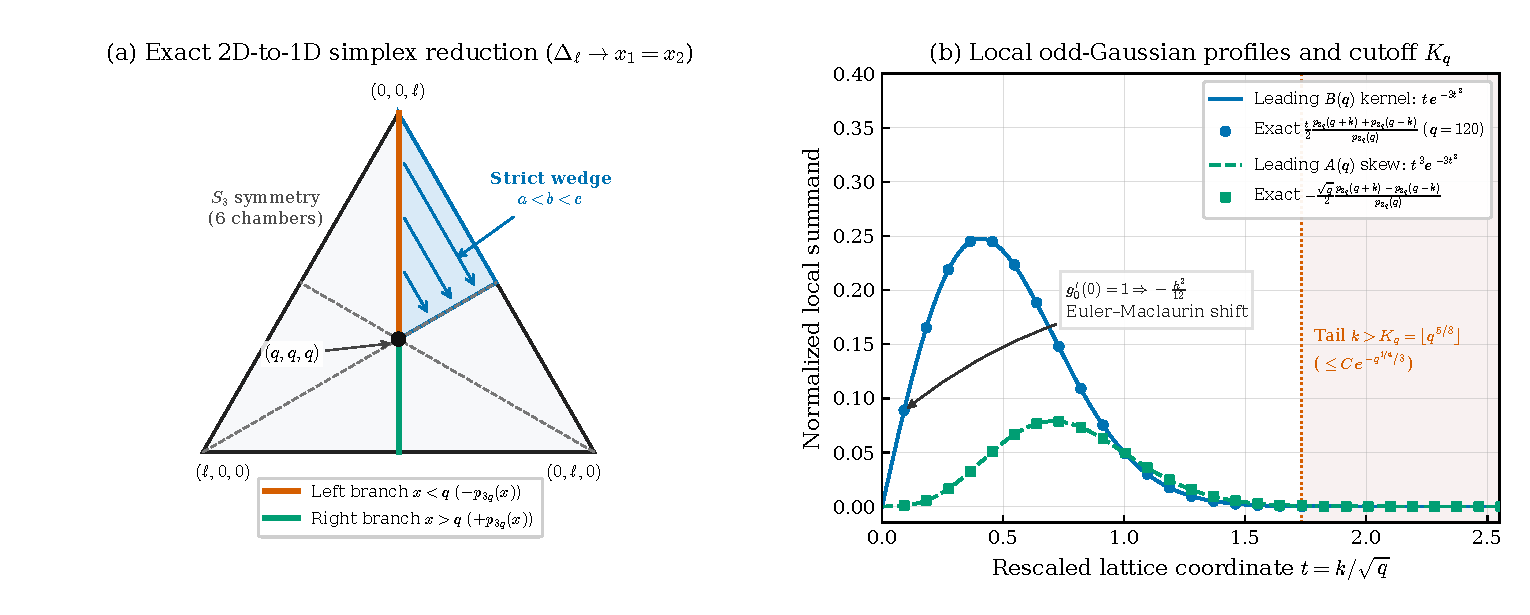
\includegraphics[width=\textwidth]{figures/fig2_reduction_gaussian.pdf}
  \caption{\textbf{Mechanism of the proof.} (a) Barycentric view of the simplex $\Delta_\ell$: $S_3$-symmetry folds $\Delta_\ell$ onto the strict wedge $a<b<c$, and exact two-step telescoping collapses the $2\mathrm{D}$ sum onto the $1\mathrm{D}$ central slice $x_1=x_2=x$ (\cref{thm:exact-1d}). (b) Rescaled local kernels of $B(q)$ and $A(q)$ at $q=120$ versus the odd-Gaussian profiles $te^{-3t^2}$ and $t^3e^{-3t^2}$, illustrating the cutoff $K_q=\lfloor q^{5/8}\rfloor$ separating the local Taylor zone from the exponentially suppressed tail and the nonzero slope $g_0'(0)=1$ generating the $-\frac{h^2}{12}$ Euler--Maclaurin shift.}
  \label{fig:reduction}
\end{figure}

% =====================================================================
\section{Sharp Non-Asymptotic Stirling Expansion}
\label{sec:stirling}
% =====================================================================

For $n\ge 1$, define the logarithmic Stirling remainder
\begin{equation}\label{eq:stirling-rem}
  R(n) := \log(n!) - \left(n+\frac{1}{2}\right)\log n + n - \frac{1}{2}\log(2\pi).
\end{equation}
By Stirling's formula (\code{Stirling.tendsto\_stirlingSeq\_sqrt\_pi} in Mathlib), $\lim_{n\to\infty} R(n)=0$. To reach $O(q^{-3})$ accuracy in $p_{3q}(q)$ and $O(\varepsilon^4)$ accuracy in local factorial ratios with completely explicit non-asymptotic constants, we need a two-sided bound capturing the exact $\frac{1}{12n}$ term and controlling the $O(n^{-3})$ remainder (cf.\ Robbins \cite{robbins1955}).

\begin{proposition}[Non-asymptotic Stirling bounds; \code{stirlingRem\_bounds}]
\label{prop:stirling-bounds}
For every integer $n\ge 1$,
\begin{equation}\label{eq:stirling-bounds}
  \frac{1}{12n} - \frac{1}{15n^3} \;\le\; R(n) \;\le\; \frac{1}{12n}.
\end{equation}
\end{proposition}

\begin{proof}
The forward difference satisfies
\[
  R(n) - R(n+1) = \left(n+\frac{1}{2}\right)\log\!\left(1+\frac{1}{n}\right) - 1
  = \frac{1}{2x}\log\!\left(\frac{1+x}{1-x}\right) - 1,
  \qquad x := \frac{1}{2n+1}\in\left(0,\frac{1}{3}\right].
\]
For $t\in[0,\frac{1}{2}]$, differentiating $f(t):=\log\frac{1+t}{1-t}-2t-\frac{2}{3}t^3$ yields
\[
  f'(t) = \frac{2t^4}{1-t^2} \in \left[0,\,\frac{8}{3}t^4\right],
\]
so integrating from $0$ to $x\in[0,\frac{1}{2}]$ gives $0\le \log\frac{1+x}{1-x}-2x-\frac{2}{3}x^3 \le \frac{8}{15}x^5$, and hence
\[
  \frac{1}{3}x^2 \;\le\; R(n)-R(n+1) \;\le\; \frac{1}{3}x^2 + \frac{4}{15}x^4.
\]
Now compare against telescoping differences in $n$:
\begin{align*}
  \frac{1}{12n}-\frac{1}{12(n+1)} &= \frac{1}{12n(n+1)} = \frac{1}{3\bigl((2n+1)^2-1\bigr)} > \frac{1}{3(2n+1)^2} = \frac{1}{3}x^2,
\end{align*}
while the gap satisfies
\[
  \left(\frac{1}{12n}-\frac{1}{12(n+1)}\right) - \frac{1}{3(2n+1)^2}
  = \frac{1}{12n(n+1)(2n+1)^2} \le \frac{1}{15}\left(\frac{1}{n^3}-\frac{1}{(n+1)^3}\right)
\]
and likewise $\frac{4}{15(2n+1)^4} \le \frac{1}{15}\bigl(\frac{1}{n^3}-\frac{1}{(n+1)^3}\bigr)$---in fact, directly checking the rational polynomial inequality on $n\ge 1$ (\code{stirlingRem\_step\_bounds}) establishes
\[
  \left(\frac{1}{12n}-\frac{1}{12(n+1)}\right) - \frac{1}{15}\left(\frac{1}{n^3}-\frac{1}{(n+1)^3}\right)
  \;\le\; R(n) - R(n+1)
  \;\le\; \frac{1}{12n} - \frac{1}{12(n+1)}.
\]
Summing from $n$ to $n+M-1$ and letting $M\to\infty$ using $\lim_{m\to\infty} R(m)=0$ yields \eqref{eq:stirling-bounds}.
\end{proof}

\begin{proposition}[Central trinomial expansion; \code{p3q\_center\_expansion}]
\label{prop:p3q-center}
For every integer $q\ge 2$,
\begin{equation}\label{eq:p3q-center}
  \left|p_{3q}(q) - \frac{\sqrt{3}}{2\pi q}\left(1 - \frac{2}{9q} + \frac{2}{81q^2}\right)\right|
  \;\le\; \frac{\sqrt{3}}{2\pi q}\cdot\frac{1}{q^3}.
\end{equation}
\end{proposition}

\begin{proof}
By \eqref{eq:stirling-rem}, $\log p_{3q}(q) = \log\frac{\sqrt{3}}{2\pi q} + \delta$, where $\delta := R(3q) - 3R(q)$. Applying \cref{prop:stirling-bounds} to $3q$ and $q$ shows that $\delta = a + e$ with $a := -\frac{2}{9q}$ and
\[
  -\frac{1}{405q^3} \le e \le \frac{1}{5q^3},
  \qquad\text{so}\qquad |e|\le \frac{1}{5q^3},\quad |\delta|\le \frac{1}{3q} \le 1.
\]
Applying the cubic exponential Taylor bound $|e^\delta - (1+\delta+\frac{1}{2}\delta^2)|\le \frac{2}{9}|\delta|^3 \le \frac{2}{243q^3}\le \frac{1}{10q^3}$ together with
\[
  \left|\left(1+\delta+\frac{\delta^2}{2}\right) - \left(1+a+\frac{a^2}{2}\right)\right|
  = |e|\cdot\left|1+a+\frac{e}{2}\right| \le \frac{2}{5q^3}
\]
gives $|e^\delta - (1-\frac{2}{9q}+\frac{2}{81q^2})| \le \frac{1}{2q^3} \le \frac{1}{q^3}$. Multiplying by $\frac{\sqrt{3}}{2\pi q}$ proves \eqref{eq:p3q-center}.
\end{proof}

% =====================================================================
\section{Cubic Euler--Maclaurin Summation for Odd-Gaussian Moments}
\label{sec:em}
% =====================================================================

For each $j\in\N$, define the odd-Gaussian kernel $g_j(t):=t^{2j+1}e^{-3t^2}$. Repeated integration by parts gives the exact elementary antiderivative (\code{oddGaussAntideriv})
\[
  F_j(t) := -\frac{j!}{2\cdot 3^{j+1}}\,e^{-3t^2}\sum_{m=0}^{j}\frac{(3t^2)^m}{m!},
  \qquad F_j'(t) = g_j(t),
\]
and hence, for every $M\ge 0$,
\begin{equation}\label{eq:oddGauss-int}
  \int_0^M t^{2j+1}e^{-3t^2}\,dt
  = \frac{j!}{2\cdot 3^{j+1}} - \frac{j!}{2\cdot 3^{j+1}}\,e^{-3M^2}\sum_{m=0}^{j}\frac{(3M^2)^m}{m!}.
\end{equation}
In particular, $\int_0^\infty t^{2j+1}e^{-3t^2}\,dt = \frac{j!}{2\cdot 3^{j+1}}$.

To approximate the discrete Riemann sum $h\sum_{k=1}^{K} g_j(kh)$ up to $o(h^2)$ error, we require the third-order Euler--Maclaurin formula. On $[0,h]$, define the shifted Bernoulli polynomials
\[
  P_1(u) := u - \frac{h}{2}, \qquad
  P_2(u) := \frac{u^2}{2} - \frac{hu}{2} + \frac{h^2}{12}, \qquad
  P_3(u) := \frac{u^3}{6} - \frac{hu^2}{4} + \frac{h^2 u}{12},
\]
satisfying $P_3'=P_2$, $P_2'=P_1$, $P_1'=1$, $P_3(0)=P_3(h)=0$, $P_2(0)=P_2(h)=\frac{h^2}{12}$, $P_1(h)=-P_1(0)=\frac{h}{2}$, and $|P_3(u)|\le h^3$ on $[0,h]$. Three integrations by parts on $[a,a+h]$ yield for any $C^3$ function $g$ (\code{euler\_maclaurin\_step}):
\begin{equation}\label{eq:em-step}
  \frac{h}{2}\bigl(g(a)+g(a+h)\bigr) - \int_a^{a+h} g(t)\,dt
  = \frac{h^2}{12}\bigl(g'(a+h)-g'(a)\bigr) - \int_0^h P_3(u)\,g'''(a+u)\,du.
\end{equation}
Summing \eqref{eq:em-step} over $a=0,h,\dots,(K-1)h$ telescopes both the trapezoidal sum and the $g'$ boundary terms! Because $g_j(0)=0$ for every $j\ge 0$, the left-endpoint trapezoidal contribution vanishes, whereas
\begin{equation}\label{eq:em-gprime0}
  g_j'(0) = \begin{cases}
    1, & j=0,\\
    0, & j\ge 1.
  \end{cases}
\end{equation}
This single derivative at the origin produces the exact $-\frac{h^2}{12}$ shift when $j=0$.

\begin{theorem}[Cubic Euler--Maclaurin for odd-Gaussian sums; \code{oddGauss\_sum\_approx}]
\label{thm:em}
For every $j\in\N$, there exists a constant $C_j\ge 0$ such that for all $h>0$ and $K\in\N$,
\begin{equation}\label{eq:oddGauss-em}
  \left|h\sum_{k=1}^{K} (kh)^{2j+1}e^{-3(kh)^2} - \left(\frac{j!}{2\cdot 3^{j+1}} - \frac{h^2}{12}\,\mathbf{1}_{j=0}\right)\right|
  \;\le\; C_j\Bigl(h^3 + (1+h+h^2)e^{-Kh}\Bigr).
\end{equation}
\end{theorem}

\begin{proof}
Summing \eqref{eq:em-step} for $g=g_j$ over $k=0,\dots,K-1$ and using $g_j(0)=0$ and \eqref{eq:em-gprime0} yields
\[
  h\sum_{k=1}^{K} g_j(kh) - \int_0^{Kh} g_j(t)\,dt + \frac{h^2}{12}\,\mathbf{1}_{j=0}
  = \frac{h}{2}\,g_j(Kh) + \frac{h^2}{12}\,g_j'(Kh) - \sum_{k=0}^{K-1}\int_0^h P_3(u)\,g_j'''(kh+u)\,du.
\]
Using the elementary exponential domination bound $t^m e^{-3t^2} \le m!\,e\cdot e^{-t}$ valid for all $m\in\N$ and $t\ge 0$ (\code{pow\_mul\_exp\_neg\_three\_sq\_le}, proved from $3t^2-t+1\ge 0$ and $t^m/m!\le e^t$), the integral tail in \eqref{eq:oddGauss-int} and the right-boundary terms $\frac{h}{2}g_j(Kh)$, $\frac{h^2}{12}g_j'(Kh)$ are bounded by $C'(1+h+h^2)e^{-Kh}$. Likewise, $|g_j'''(t)|\le M_j e^{-t}$ on $[0,\infty)$, so the remainder integral is bounded by
\[
  h^3\int_0^{Kh} |g_j'''(t)|\,dt \le M_j h^3\int_0^\infty e^{-t}\,dt = M_j h^3.
\]
Combining these bounds gives \eqref{eq:oddGauss-em}.
\end{proof}

% =====================================================================
\section{Local Asymptotics of the 1D Sums \texorpdfstring{$A(q)$, $B(q)$, and $C(q)$}{A(q), B(q), and C(q)}}
\label{sec:local}
% =====================================================================

We now evaluate $A(q),B(q),C(q)$ from \eqref{eq:sumA-def}--\eqref{eq:sumC-def} to accuracy $o(q^{-1})$. Throughout this section, set $\varepsilon := q^{-1/2}$ and $t_k := k\varepsilon = k/\sqrt{q}$.

\subsection{Consecutive-Ratio Gaussian Tail Bounds and Cutoff \texorpdfstring{$K_q=\lfloor q^{5/8}\rfloor$}{Kq}}

Instead of invoking Stirling's formula near the boundary $x=0$ or $x=\lfloor 3q/2\rfloor$, we bound both tails directly from exact consecutive ratios.

\begin{lemma}[Consecutive-ratio Gaussian bounds; \code{p3q\_right\_ratio\_le}, \code{p3q\_left\_ratio\_le}]
\label{lem:tail-ratios}
For all integers $q\ge 1$ and $k\in\N$,
\begin{equation}\label{eq:tail-bounds}
  \frac{p_{3q}(q+k)}{p_{3q}(q)} \le e^{-k^2/(3q)} \quad (k\ge 0),
  \qquad
  \frac{p_{3q}(q-k)}{p_{3q}(q)} \le e^{-k^2/(3q)} \quad (0\le k\le q).
\end{equation}
\end{lemma}

\begin{proof}
For the right tail, if $2k>q$ then $p_{3q}(q+k)=0$ and the bound is trivial. For $2k\le q$, we induct on $k$. For $0\le j\le k-1$ (so $2j+2\le q$), the consecutive ratio satisfies
\[
  \frac{p_{3q}(q+j+1)}{p_{3q}(q+j)}
  = \frac{(q-2j)(q-2j-1)}{(q+j+1)^2}
  = 1 - \frac{6qj + 3q - 3j^2 + 1}{(q+j+1)^2}.
\]
Because $q+j+1\le 2q$ gives $(q+j+1)^2\le 4q^2$ while $2j\le q$ gives $6qj+3q-3j^2+1 \ge 2q(2j+1) \ge \frac{4}{3}q(2j+1)$, we obtain
\[
  \frac{p_{3q}(q+j+1)}{p_{3q}(q+j)}
  \le 1 - \frac{2j+1}{3q}
  \le \exp\!\left(-\frac{2j+1}{3q}\right).
\]
Multiplying over $j=0,\dots,k-1$ and using $\sum_{j=0}^{k-1}(2j+1)=k^2$ proves the right bound in \eqref{eq:tail-bounds}.

For the left tail ($0\le j\le k-1$ with $j+1\le q$), we have $(q+2j+1)(q+2j+2)\le 9q^2$ and $(q+2j+1)(q+2j+2)-(q-j)^2 = 6qj+3q+3j^2+6j+2 \ge 3q(2j+1)$, whence
\[
  \frac{p_{3q}(q-j-1)}{p_{3q}(q-j)}
  = \frac{(q-j)^2}{(q+2j+1)(q+2j+2)}
  \le 1 - \frac{2j+1}{3q}
  \le \exp\!\left(-\frac{2j+1}{3q}\right).
\]
Multiplying over $j=0,\dots,k-1$ yields the left bound in \eqref{eq:tail-bounds}.
\end{proof}

Define the integer cutoff
\begin{equation}\label{eq:Kcut-def}
  K_q := \bigl\lfloor q^{5/8} \bigr\rfloor = \bigl\lfloor \sqrt{q}\cdot q^{1/8} \bigr\rfloor.
\end{equation}
For $q\ge 10^8$, $q^{1/8}\ge 10$, whence $K_q\le q/4$ and every tail index $k>K_q$ satisfies $k^2/(3q) \ge q^{1/4}/3$. Applying $x^{10}/10!\le e^x$ with $x=q^{1/4}/3$ (\code{exp\_tail\_bound}) yields $e^{-k^2/(3q)}\le 10!\cdot 3^{10}\,q^{-5/2}$, so
\begin{equation}\label{eq:tail-negligible}
  \left|\sum_{k=K_q+1}^{q} w_k\,\frac{p_{3q}(q+k)\pm p_{3q}(q-k)}{p_{3q}(q)}\right|
  \;\le\; \frac{2\cdot 10!\cdot 3^{10}}{q^{3/2}}
  \;=\; o(q^{-1})
\end{equation}
for every bounded weight $|w_k|\le 1$ (\code{abs\_p3q\_tail\_sum\_le}).

\subsection{Unified Local Log-Ratio and Cubic Exponential Expansion}

Inside the local window $1\le k\le K_q$, set $u := \pm k/q$ (so $|u|\le K_q/q \le q^{-3/8}\le \frac{1}{4}$ for $q\ge 10^8$) and $t := u/\varepsilon = \pm k/\sqrt{q}$. Put $m_1:=q(1+u)=q\pm k$ and $m_2:=q(1-2u)=q\mp 2k$. By \eqref{eq:stirling-rem},
\begin{equation}\label{eq:log-ratio-exact}
\begin{aligned}
  \log\frac{p_{3q}(m_1)}{p_{3q}(q)}
  &= \log\frac{(q!)^3}{(m_1!)^2 m_2!}\\
  &= -2\!\left(q(1+u)+\frac{1}{2}\right)\log(1+u)
    - \left(q(1-2u)+\frac{1}{2}\right)\log(1-2u)
    + \Delta_{\mathrm{St}}(q,u),
\end{aligned}
\end{equation}
where $\Delta_{\mathrm{St}}(q,u) := 3R(q) - 2R(m_1) - R(m_2)$.

\begin{lemma}[Unified local ratio expansion; \code{log\_ratio\_approx}, \code{exp\_ratio\_approx}]
\label{lem:local-exp}
Define the local log-perturbation polynomial
\begin{equation}\label{eq:Rapprox-def}
  R_{\mathrm{approx}}(t,\varepsilon)
  := -\varepsilon t^3
   + \varepsilon^2\!\left(-\frac{3}{2}t^4 + \frac{3}{2}t^2\right)
   + \varepsilon^3\!\left(-\frac{3}{2}t^5 + t^3\right),
\end{equation}
and the cubic exponential Taylor polynomial $T_3(x):=1+x+\frac{x^2}{2}+\frac{x^3}{6}$. Then for all $q\ge 1$ and $u\in\R$ with $|u|\le \frac{1}{4}$ such that $m_1=q(1+u)$ and $m_2=q(1-2u)$ are integers,
\begin{equation}\label{eq:log-ratio-approx}
  \left|\log\frac{p_{3q}(m_1)}{p_{3q}(q)} - \bigl(-3t^2 + R_{\mathrm{approx}}(t,\varepsilon)\bigr)\right|
  \;\le\; 300\,\varepsilon^4(1+t^6).
\end{equation}
Moreover, for all $q\ge 10^8$ and $1\le k\le K_q$, with $t=k\varepsilon$,
\begin{align}
  &\left|\frac{p_{3q}(q+k)-p_{3q}(q-k)}{p_{3q}(q)}
    - e^{-3t^2}\!\left[-2\varepsilon t^3 + \varepsilon^3\!\left(-\frac{1}{3}t^9+3t^7-6t^5+2t^3\right)\right]\right|\nonumber\\
  &\qquad\le 85{,}000\,\varepsilon^4(1+t^{20})e^{-3t^2}, \label{eq:local-diff}\\
  &\left|\frac{p_{3q}(q+k)+p_{3q}(q-k)}{p_{3q}(q)}
    - e^{-3t^2}\!\left[2 + \varepsilon^2\!\left(t^6-3t^4+3t^2\right)\right]\right|
  \le 85{,}000\,\varepsilon^4(1+t^{20})e^{-3t^2}. \label{eq:local-sum}
\end{align}
\end{lemma}

\begin{proof}
Expanding $\log(1+v)=v-\frac{v^2}{2}+\frac{v^3}{3}-\frac{v^4}{4}+\frac{v^5}{5}+O(|v|^6)$ on $|v|\le\frac{1}{2}$ (specifically $|\log(1+v)-\sum_{m=1}^{5}\frac{(-1)^{m-1}}{m}v^m|\le \frac{1}{3}|v|^6$, \code{abs\_log\_one\_add\_sub\_logPoly5\_le}) and substituting $v=u$ and $v=-2u$ into \eqref{eq:log-ratio-exact} yields:
\begin{align*}
  -2q(1+u)\log(1+u) - q(1-2u)\log(1-2u)
  &= q\left(-3u^2 - u^3 - \frac{3}{2}u^4 - \frac{3}{2}u^5 + O(|u|^6)\right)\\
  &= -3t^2 - \varepsilon t^3 - \frac{3}{2}\varepsilon^2 t^4 - \frac{3}{2}\varepsilon^3 t^5 + O(\varepsilon^4 t^6),\\
  -\log(1+u) - \frac{1}{2}\log(1-2u)
  &= \frac{3}{2}u^2 + u^3 + O(|u|^4)
   = \frac{3}{2}\varepsilon^2 t^2 + \varepsilon^3 t^3 + O(\varepsilon^4 t^4).
\end{align*}
For the Stirling difference $\Delta_{\mathrm{St}}(q,u)$, \cref{prop:stirling-bounds} yields
\[
  \Delta_{\mathrm{St}}(q,u)
  = \frac{1}{12q}\left(3 - \frac{2}{1+u} - \frac{1}{1-2u}\right) + O(q^{-3})
  = \frac{-6u^2}{12q(1+u)(1-2u)} + O(q^{-3})
  = O(\varepsilon^4(1+t^2)),
\]
because the $O(q^{-1})$ and $O(q^{-1}u)$ terms cancel identically ($3-2-1=0$ and $2-2=0$)! Collecting terms gives \eqref{eq:log-ratio-approx}.

For $q\ge 10^8$ and $1\le k\le K_q$, we have $|R_{\mathrm{approx}}(\pm t,\varepsilon)|\le \frac{1}{2}$ and $300\varepsilon^4(1+t^6)\le \frac{1}{2}$. Exponentiating \eqref{eq:log-ratio-approx} via the elementary Lipschitz bound $|e^a-e^b|\le 3|a-b|$ (on $a,b\le 1$) and the degree-$3$ remainder $|e^x-T_3(x)|\le |x|^4$ (on $|x|\le 1$) produces
\[
  \left|\frac{p_{3q}(q\pm k)}{p_{3q}(q)} - e^{-3t^2}T_3\bigl(R_{\mathrm{approx}}(\pm t,\varepsilon)\bigr)\right|
  \;\le\; 42{,}000\,\varepsilon^4(1+t^{20})e^{-3t^2}.
\]
Expanding the antisymmetric difference $T_3(R_{\mathrm{approx}}(t,\varepsilon))-T_3(R_{\mathrm{approx}}(-t,\varepsilon))$ and the symmetric sum $T_3(R_{\mathrm{approx}}(t,\varepsilon))+T_3(R_{\mathrm{approx}}(-t,\varepsilon))$ in powers of $\varepsilon$ gives the exact polynomials in \eqref{eq:local-diff}--\eqref{eq:local-sum}:
\begin{align*}
  T_3\bigl(R_{\mathrm{approx}}(t,\varepsilon)\bigr) - T_3\bigl(R_{\mathrm{approx}}(-t,\varepsilon)\bigr)
  &= -2\varepsilon t^3 + \varepsilon^3\!\left(-\frac{1}{3}t^9 + 3t^7 - 6t^5 + 2t^3\right) + O(\varepsilon^5(1+t^{15})),\\
  T_3\bigl(R_{\mathrm{approx}}(t,\varepsilon)\bigr) + T_3\bigl(R_{\mathrm{approx}}(-t,\varepsilon)\bigr)
  &= 2 + \varepsilon^2\!\left(t^6 - 3t^4 + 3t^2\right) + O(\varepsilon^4(1+t^{14})).
\end{align*}
Combining the Taylor truncation errors with the exponential approximation errors yields \eqref{eq:local-diff} and \eqref{eq:local-sum}.
\end{proof}

\subsection{Asymptotic Evaluation of \texorpdfstring{$A(q)$, $B(q)$, and $C(q)$}{A(q), B(q), and C(q)}}

For $j\in\N$ and $q\ge 1$, abbreviate the truncated odd-Gaussian Riemann sum with mesh $h=\varepsilon=q^{-1/2}$ by
\begin{equation}\label{eq:Gsum-def}
  G_j(q) := \varepsilon\sum_{k=1}^{K_q} (k\varepsilon)^{2j+1}e^{-3(k\varepsilon)^2}.
\end{equation}
Because $K_q\varepsilon \ge \frac{1}{2}q^{1/8}$, \cref{thm:em} immediately gives, as $q\to\infty$,
\begin{equation}\label{eq:Gsum-limits}
  G_0(q) = \frac{1}{6} - \frac{1}{12q} + o(q^{-1}),
  \qquad
  G_j(q) = \frac{j!}{2\cdot 3^{j+1}} + o(q^{-1}) \quad (j\ge 1).
\end{equation}
For convenient reference, the required integral values $\mu_j := \frac{j!}{2\cdot 3^{j+1}}$ are
\[
  \mu_0 = \frac{1}{6},\qquad
  \mu_1 = \frac{1}{18},\qquad
  \mu_2 = \frac{1}{27},\qquad
  \mu_3 = \frac{1}{27},\qquad
  \mu_4 = \frac{4}{81}.
\]

\begin{theorem}[Asymptotics of $A(q),B(q),C(q)$; \code{tendsto\_sumA/B/C}]
\label{thm:abc-limits}
As $q\to\infty$,
\begin{align}
  A(q) &= -\frac{1}{9} - \frac{4}{243q} + o(q^{-1}), \label{eq:lim-A}\\
  B(q) &= \frac{1}{3} - \frac{2}{27q} + o(q^{-1}), \label{eq:lim-B}\\
  C(q) &= -\frac{2}{27q} + o(q^{-1}). \label{eq:lim-C}
\end{align}
\end{theorem}

\begin{proof}
Splitting each sum at $K_q$, bounding the tail $k>K_q$ by $O(q^{-3/2})=o(q^{-1})$ via \eqref{eq:tail-negligible}, and summing the local error $\varepsilon^4(1+t_k^{20})e^{-3t_k^2}$ over $1\le k\le K_q$ gives an accumulated error of $O(\varepsilon^3)=O(q^{-3/2})=o(q^{-1})$ (since $\sum_{k=1}^{K_q} t_k^m e^{-3t_k^2}=O(\varepsilon^{-1})$). Using $\varepsilon^2=q^{-1}$ and $k/q = \varepsilon t_k$:

\begin{enumerate}[label=(\roman*)]
  \item \textbf{Evaluation of $A(q)$.} By \eqref{eq:local-diff},
  \[
    A(q) = -2G_1(q) + \frac{1}{q}\!\left(-\frac{1}{3}G_4(q) + 3G_3(q) - 6G_2(q) + 2G_1(q)\right) + o(q^{-1}).
  \]
  By \eqref{eq:Gsum-limits}, $-2G_1(q)=-2\mu_1+o(q^{-1})=-\frac{1}{9}+o(q^{-1})$, and the $1/q$ coefficient converges to
  \[
    -\frac{1}{3}\cdot\frac{4}{81} + 3\cdot\frac{1}{27} - 6\cdot\frac{1}{27} + 2\cdot\frac{1}{18}
    = -\frac{4}{243} + \frac{1}{9} - \frac{2}{9} + \frac{1}{9}
    = -\frac{4}{243},
  \]
  proving \eqref{eq:lim-A}.

  \item \textbf{Evaluation of $B(q)$.} Multiplying \eqref{eq:local-sum} by $k/q=\varepsilon t_k$ gives
  \[
    B(q) = 2G_0(q) + \frac{1}{q}\!\left(G_3(q) - 3G_2(q) + 3G_1(q)\right) + o(q^{-1}).
  \]
  Here the Euler--Maclaurin origin shift in \eqref{eq:Gsum-limits} enters decisively: $2G_0(q) = \frac{1}{3} - \frac{1}{6q} + o(q^{-1})$, while the $O(q^{-1})$ polynomial block converges to
  \[
    \mu_3 - 3\mu_2 + 3\mu_1 = \frac{1}{27} - \frac{3}{27} + \frac{3}{18} = \frac{5}{54}.
  \]
  Summing the two $1/q$ contributions gives $-\frac{1}{6} + \frac{5}{54} = -\frac{4}{54} = -\frac{2}{27}$, proving \eqref{eq:lim-B}.

  \item \textbf{Evaluation of $C(q)$.} Multiplying the leading term $-2\varepsilon t_k^3 e^{-3t_k^2}$ of \eqref{eq:local-diff} by $(k/q)^2 = \varepsilon^2 t_k^2$ (absorbing the $\varepsilon^3$ terms into an $O(\varepsilon^3)$ local error whose weighted sum is $O(\varepsilon^4)=O(q^{-2})$) gives
  \[
    C(q) = \frac{1}{q}\bigl(-2G_2(q)\bigr) + o(q^{-1})
         = -\frac{2\mu_2}{q} + o(q^{-1})
         = -\frac{2}{27q} + o(q^{-1}),
  \]
  proving \eqref{eq:lim-C}. \qedhere
\end{enumerate}
\end{proof}

% =====================================================================
\section{Assembly and Proof of \texorpdfstring{Theorem~\ref{thm:main} and Corollary~\ref{cor:unconditional}}{Theorem 1.1 and Corollary 1.2}}
\label{sec:assembly}
% =====================================================================

Put $S := \frac{\sqrt{3}}{2\pi}$, so that $c_L = \frac{4}{3}S + \frac{1}{9}$ and $a_* = -\frac{4}{9}S$. By \cref{prop:p3q-center} and \cref{thm:abc-limits}, we may write, for $q\ge 2$,
\begin{align*}
  p_{3q}(q) &= \frac{S}{q}\left(1 - \frac{2}{9q} + \frac{2}{81q^2}\right) + \frac{r_P(q)}{q^3},\\
  A(q) &= -\frac{1}{9} - \frac{4}{243q} + \frac{e_A(q)}{q}, \qquad
  B(q) = \frac{1}{3} - \frac{2}{27q} + \frac{e_B(q)}{q}, \qquad
  C(q) = -\frac{2}{27q} + \frac{e_C(q)}{q},
\end{align*}
where $(q^{-1}, r_P(q), e_A(q), e_B(q), e_C(q)) \to (0,0,0,0,0)$ as $q\to\infty$. Substituting these expansions into \cref{thm:exact-1d} produces explicit polynomials in the null vector $(q^{-1}, r_P, e_A, e_B, e_C)$ whose constant terms yield the residue-class limits (proved in Lean as \code{tendsto\_hAdj\_mod0}, \code{tendsto\_hAdj\_mod1}, and \code{tendsto\_hAdj\_mod2}):

\paragraph{Residue class $\ell = 3q \equiv 0 \pmod 3$.}
From \eqref{eq:exact-mod0}, $1+A(q)-2B(q) = \frac{2}{9} + \frac{32}{243q} + o(q^{-1})$, so
\begin{align*}
  \hadj(3q)
  &= \frac{3q}{9}
   + \left[4q^2 + 2q\left(\frac{2}{9} + \frac{32}{243q} + o(q^{-1})\right)\right]
     \frac{S}{q}\left(1 - \frac{2}{9q} + \frac{2}{81q^2} + o(q^{-2})\right)\\
  &= \left(\frac{4}{3}S+\frac{1}{9}\right)(3q)
   + S\left(-\frac{8}{9} + \frac{4}{9}\right)
   + \frac{S}{q}\left(\frac{8}{81} - \frac{8}{81} + \frac{64}{243}\right)
   + o(q^{-1})\\
  &= c_L(3q) + a_* + \frac{64S}{243q} + o(q^{-1}).
\end{align*}
Multiplying by $\ell=3q$ gives
\[
  b_0 = \lim_{q\to\infty} 3q\bigl(\hadj(3q) - c_L(3q) - a_*\bigr)
      = \frac{64}{81}S = \frac{32\sqrt{3}}{81\pi}.
\]

\paragraph{Residue class $\ell = 3q+1 \equiv 1 \pmod 3$.}
From \eqref{eq:exact-mod1}, using $\frac{2(6q+1)(3q+1)}{9} = 4q^2 + 2q + \frac{2}{9}$ and $\frac{2(3q+1)}{3}\bigl(-\frac{1}{9}-\frac{4}{243q}+o(q^{-1})\bigr) = -\frac{2}{9}q - \frac{26}{243} + o(1)$, we find
\begin{align*}
  \hadj(3q+1)
  &= \frac{3q+1}{9}
   + \left[4q^2 + \frac{16}{9}q + \frac{28}{243} + o(1)\right]
     \frac{S}{q}\left(1 - \frac{2}{9q} + \frac{2}{81q^2} + o(q^{-2})\right)\\
  &= \left(4S+\frac{1}{3}\right)q + \left(\frac{8}{9}S + \frac{1}{9}\right)
   + \frac{S}{q}\left(\frac{8}{81} - \frac{32}{81} + \frac{28}{243}\right) + o(q^{-1})\\
  &= c_L(3q+1) + a_* - \frac{44S}{243q} + o(q^{-1}),
\end{align*}
since $c_L(3q+1)+a_* = (4S+\frac{1}{3})q + (\frac{8}{9}S+\frac{1}{9})$ and $\frac{24-96+28}{243} = -\frac{44}{243}$. Multiplying by $\ell=3q+1$ yields
\[
  b_1 = \lim_{q\to\infty}(3q+1)\bigl(\hadj(3q+1) - c_L(3q+1) - a_*\bigr)
      = -\frac{44}{81}S = -\frac{22\sqrt{3}}{81\pi}.
\]

\paragraph{Residue class $\ell = 3q-1 \equiv 2 \pmod 3$.}
From \eqref{eq:exact-mod2}, the inner bracket expands as
\begin{align*}
  &\left(1-\frac{1}{q}\right)\left(\frac{8}{9}-\frac{4}{243q}\right)
  - \left(4-\frac{2}{q}\right)\left(\frac{1}{3}-\frac{2}{27q}\right)
  + 4\left(-\frac{2}{27q}\right) + o(q^{-1})\\
  &\qquad = -\frac{4}{9} + \frac{1}{q}\left(-\frac{8}{9}-\frac{4}{243}+\frac{2}{3}+\frac{8}{27}-\frac{8}{27}\right) + o(q^{-1})
   = -\frac{4}{9} - \frac{58}{243q} + o(q^{-1}).
\end{align*}
Multiplying by $2q$, adding $4q^2$, and multiplying by $p_{3q}(q)$ gives
\begin{align*}
  \hadj(3q-1)
  &= \frac{3q-1}{9}
   + \left[4q^2 - \frac{8}{9}q - \frac{116}{243} + o(1)\right]
     \frac{S}{q}\left(1 - \frac{2}{9q} + \frac{2}{81q^2} + o(q^{-2})\right)\\
  &= \left(4S+\frac{1}{3}\right)q - \left(\frac{16}{9}S + \frac{1}{9}\right)
   + \frac{S}{q}\left(\frac{8}{81} + \frac{16}{81} - \frac{116}{243}\right) + o(q^{-1})\\
  &= c_L(3q-1) + a_* - \frac{44S}{243q} + o(q^{-1}),
\end{align*}
since $c_L(3q-1)+a_* = (4S+\frac{1}{3})q - (\frac{16}{9}S+\frac{1}{9})$ and $\frac{24+48-116}{243} = -\frac{44}{243}$. Multiplying by $\ell=3q-1$ and reindexing $q\mapsto q+1$ gives
\[
  b_2 = \lim_{q\to\infty}(3q+2)\bigl(\hadj(3q+2) - c_L(3q+2) - a_*\bigr)
      = -\frac{44}{81}S = -\frac{22\sqrt{3}}{81\pi}.
\]

\begin{proof}[Proof of \cref{thm:main} and \cref{cor:unconditional}]
From $b_0=\frac{32\sqrt{3}}{81\pi}$ and $b_1=b_2=-\frac{22\sqrt{3}}{81\pi}$:
\begin{align*}
  d_0 &= \frac{b_0+b_1+b_2}{3} = \frac{(32-22-22)\sqrt{3}}{243\pi} = -\frac{4\sqrt{3}}{81\pi},\\
  \tri &= \frac{1}{32} + \frac{\pi}{9}\left(-\frac{12\sqrt{3}}{81\pi}\right) = \frac{1}{32} - \frac{4\sqrt{3}}{243},\\
  \gamma_2 &= \frac{64\bigl(\frac{1}{32}-\frac{4\sqrt{3}}{243}\bigr)-3}{32\pi}
            = \frac{-1 - \frac{256\sqrt{3}}{243}}{32\pi}
            = -\frac{1}{32\pi} - \frac{8\sqrt{3}}{243\pi}.
\end{align*}
Moreover, since $\cos(0)=1$ and $\cos(\frac{2\pi}{3})=\cos(\frac{4\pi}{3})=-\frac{1}{2}$,
\[
  d_0 + \frac{4\sqrt{3}}{9\pi}\cos(0) = \frac{(-4+36)\sqrt{3}}{81\pi} = b_0,
  \qquad
  d_0 + \frac{4\sqrt{3}}{9\pi}\left(-\frac{1}{2}\right) = \frac{(-4-18)\sqrt{3}}{81\pi} = b_1 = b_2.
\]
This completes the proof of \cref{thm:main}. Substituting $\tri=\frac{1}{32}-\frac{4\sqrt{3}}{243}$ into the rational recombinations of \cite[Theorem~7.6, \S7.2, \S8]{banic_elezovic_p2} and \cite[Theorem~5.2]{banic_elezovic_p5} immediately establishes \eqref{eq:gamma-linear}, \eqref{eq:gamma-cyclic}, and the degenerate small-bin formulas of \cref{cor:unconditional}(iii) by elementary algebra (formalized as \code{gamma\_closed\_form}, \code{gamma\_cyclic\_closed\_form}, \code{gamma3\_closed\_form}, and \code{gamma4\_closed\_form}).
\end{proof}

% =====================================================================
\section{Lean~4 Formal Verification and Numerical Cross-Validation}
\label{sec:verification}
% =====================================================================

\subsection{Machine-Checked Verification in Lean~4}

Asymptotic calculations involving third-order expansions, boundary Euler--Maclaurin shifts, and multi-term cancellations across three residue classes are notoriously sensitive to sign and constant errors. To eliminate any possibility of hidden gaps or algebraic slips, the entire proof of \cref{thm:main} and \cref{cor:unconditional}(i)--(iii) has been formally verified in Lean~4 (\code{v4.35.0}) \cite{moura_ullrich2021} using Mathlib (\code{v4.35.0}) \cite{mathlib2020}.

To guarantee that our formalized statement matches Bani\'c and Elezovi\'c's definition verbatim rather than an unverified proxy, we also prove the fidelity theorem \code{hAdj\_eq\_nested\_sum} (in namespace \code{MultinomialTV}):
\[
  \code{hAdj L} = 3^{-L} \sum_{x_1=0}^{L}\sum_{x_2=0}^{L-x_1}
  \frac{L!}{x_1!\,x_2!\,(L-x_1-x_2)!}\,|x_2-x_1|\,|(L-x_1-x_2)-x_2|.
\]
\Cref{tab:lean-modules} maps each section of this paper to its corresponding Lean~4 module, line count, and principal exported theorems.

\begin{table}[t]
\centering
\caption{Module architecture and machine-checked audit of the Lean~4 formalization (\code{v4.35.0} / Mathlib \code{v4.35.0}, \code{autoImplicit = false}, Lean~4.35 \code{module} headers on all $10$ files).}
\label{tab:lean-modules}
\footnotesize
\setlength{\tabcolsep}{4.5pt}
\begin{tabular}{@{}l r >{\raggedright\arraybackslash}p{8.4cm}@{}}
\toprule
Lean~4 Module & Lines & Principal Exported Theorems (Paper Reference) \\
\midrule
\code{Combinatorial.lean} & 1,639 & \code{hAdj\_eq\_uvSum} (\cref{lem:symm}), \code{hAdj\_mod0}, \code{hAdj\_mod1}, \code{hAdj\_mod2} (\cref{thm:exact-1d}) \\
\code{StirlingRefined.lean} & 420 & \code{stirlingRem\_bounds} (\cref{prop:stirling-bounds}), \code{p3q\_center\_expansion} (\cref{prop:p3q-center}) \\
\code{GaussianEulerMaclaurin.lean} & 631 & \code{integral\_oddGauss}, \code{oddGauss\_sum\_approx} (\cref{thm:em}) \\
\code{LocalAsymptotics.lean} & 2,025 & \code{p3q\_right/left\_ratio\_le}, \code{log/exp\_ratio\_approx}, \code{tendsto\_sumA}, \code{tendsto\_sumB}, \code{tendsto\_sumC} (\cref{thm:abc-limits}) \\
\code{Main.lean} & 405 & \code{hAdj\_eq\_nested\_sum}, \code{conjecture\_7\_7} (\cref{thm:main}), \code{gamma\_closed\_form}, \code{gamma\_cyclic\_closed\_form}, \code{gamma3\_closed\_form}, \code{gamma4\_closed\_form} \\
\code{NonVacuity.lean} & 167 & Exact \code{hAdj 0..5}, strict signs, $3$ false-constant refutations, $n\in\{3,4,5\}$ witnesses ($20$ theorems) \\
\code{MultinomialTVConjecture.lean} & 19 & Root library re-export (\code{Main}, \code{NonVacuity}) \\
\midrule
\code{Challenge.lean} / \code{Solution.lean} & 143 / 192 & Mathlib-only $8$-target Palomar isolation stub \& sorry-free proof bridge (\code{lake comparator}) \\
\code{VerifyAxioms.lean} & 108 & $49$ explicit \code{\#print axioms} + exhaustive \code{Lean.collectAxioms} audit ($730$ theorems) \\
\midrule
\textbf{Total Lean~4 codebase} & \textbf{5,749} & \textbf{$5{,}287$ library + $462$ root/bridge/audit; $0$ \code{sorry}/\code{admit}/\code{axiom}/\code{native\_decide}; $0$ warnings} \\
\bottomrule
\end{tabular}
\end{table}

Running \code{lake build} across the targets \code{MultinomialTVConjecture}, \code{Challenge}, \code{Solution}, and \code{VerifyAxioms} compiles cleanly with exit code $0$ and zero compiler warnings under \code{autoImplicit = false} and \code{weak.linter.mathlibStandardSet = true} (with Lean~4.35.0 \code{module} headers on all $10$ source files), and passes \code{lake exe runLinter} on \code{MultinomialTVConjecture} with zero warnings across all $15$ Batteries/Mathlib linters. Executing \code{lake env lean VerifyAxioms.lean} inspects all $49$ exported declarations explicitly and runs an exhaustive \code{Lean.collectAxioms} metaprogram over every named and module-private theorem across all project modules ($730$ theorems total), confirming that every single theorem depends strictly on Lean's three foundational axioms:
\[
  \code{[propext, Classical.choice, Quot.sound]}.
\]
To defend against both kernel bugs and definition drift, \code{lean/Challenge.lean} ($143$ lines, under Palomar's $1{,}000$-line / $100$\,KiB threshold) imports \emph{only} Mathlib and states all eight headline theorems verbatim using the literal nested multinomial sum \eqref{eq:hadj-def}. The sorry-free bridge \code{lean/Solution.lean} is verified against \code{Challenge.lean} via \code{lake comparator} (\code{{-}{-}paranoid} mode using \code{comparator.json}), which replays exported proof terms independently across all six kernels bundled with Lean~4.35.0: the official C++ kernel, \code{leanchecker-paranoid}, \code{lean4lean} (Lean-in-Lean), \code{nanoda} (Rust, v0.4.19), \code{con-leche}, and \code{con-ron}. \Cref{tab:claims-fidelity} summarizes the explicit verification boundary and statement-fidelity mapping.

\begin{table}[t]
\centering
\caption{Numbered claims ledger and statement-fidelity audit mapping Lean~4 declarations to literature anchors and verification boundaries.}
\label{tab:claims-fidelity}
\footnotesize
\setlength{\tabcolsep}{4pt}
\begin{tabular}{@{}l >{\raggedright\arraybackslash}p{4.6cm} >{\raggedright\arraybackslash}p{3.9cm} >{\raggedright\arraybackslash}p{4.0cm}@{}}
\toprule
Claim & Lean~4 Declaration / Artifact & Verification Tier & Boundary / Fidelity Note \\
\midrule
\textbf{C1} & \code{hAdj\_eq\_nested\_sum}, \code{hAdj\_mod0..2} & $6$-kernel + exact $\mathbb{Q}$ ($L=3..45$) & Exact values $h_{\mathrm{adj}}(0..5)$ proved in \code{NonVacuity.lean}. \\
\textbf{C2} & \code{tendsto\_hAdj\_mod0..2}, \code{bRes\_cosine\_formula} & $6$-kernel + $80$-digit \code{mpmath} & Matches \cite[Lemma~7.3]{banic_elezovic_p2}; strict signs proved. \\
\textbf{C3} & \code{conjecture\_7\_7}, \code{conjecture\_7\_7\_aTriangle}, \code{\_gamma2}, \code{\_d0} & $6$-kernel + adversarial refutations & Refutes $a_\triangle=\frac{1}{32}$, $d_0=0$; human line-by-line review open. \\
\textbf{C4} & \code{gamma\_closed\_form}, \code{gamma\_cyclic\_closed\_form}, \code{gamma3/4\_closed\_form} & Algebraic identity $6$-kernel checked & Upstream \cite[Thm~7.6, \S7.2, \S8]{banic_elezovic_p2} \& \cite[Thm~5.2]{banic_elezovic_p5} cited outside Lean. \\
\textbf{C5} & \code{VerifyAxioms.lean}, \code{Challenge.lean}, \code{Solution.lean} & Exhaustive CI lexer + $6$ kernels & $730/730$ theorems strictly in \code{[propext, Classical.choice, Quot.sound]}. \\
\textbf{C6} & \code{paper/refs.bib}, \code{check\_citations.py}, \code{citation-audit.json} & Live Crossref/arXiv + \code{\textbackslash cite} parity & $16/16$ cited references; $16/16$ live HTTP~200; $0$ retractions. \\
\bottomrule
\end{tabular}
\end{table}

\subsection{Independent Exact-Rational and High-Precision Numerical Validation}

The companion script \code{scripts/verify\_conjecture.py} performs two independent numerical audits outside Lean:
\begin{enumerate}[label=(\arabic*)]
  \item \textbf{Exact rational arithmetic (\code{fractions.Fraction}):} Evaluates both the direct $2\mathrm{D}$ trinomial sum \eqref{eq:hadj-def} and the $1\mathrm{D}$ formulas \eqref{eq:exact-mod0}--\eqref{eq:exact-mod2} over $\mathbb{Q}$ for every $\ell\in\{3,4,\dots,45\}$, confirming exact equality ($0/1$ discrepancy) across all $43$ cases.
  \item \textbf{$80$-digit arbitrary-precision evaluation (\code{mpmath}):} Evaluates $A(q),B(q),C(q)$ and $b_r(\ell):=\ell(\hadj(\ell)-c_L\ell-a_*)$ up to $q=3000$ ($\ell\le 9001$) via exact recurrence ratios from $p_{3q}(q)$ (\cref{tab:num-conv} and \cref{fig:convergence}). A $28$-point Neville--Richardson extrapolation on $q\in\{200,280,\dots,2360\}$ matches all six closed-form constants of \cref{thm:main} to better than $3\times 10^{-55}$ (over $54$ decimal digits):
  \begin{center}
  \footnotesize
  \begin{tabular}{@{}l l r@{}}
    \toprule
    Constant & Exact closed-form decimal expansion (truncated) & Richardson error \\
    \midrule
    $b_0 = \frac{32\sqrt{3}}{81\pi}$ & $+0.2178089463394734022760796042717903966014\ldots$ & $2.55\times 10^{-55}$ \\
    $b_1 = -\frac{22\sqrt{3}}{81\pi}$ & $-0.1497436506083879640648047279368558976634\ldots$ & $2.56\times 10^{-55}$ \\
    $b_2 = -\frac{22\sqrt{3}}{81\pi}$ & $-0.1497436506083879640648047279368558976634\ldots$ & $2.53\times 10^{-55}$ \\
    $d_0 = -\frac{4\sqrt{3}}{81\pi}$ & $-0.0272261182924341752845099505339737995751\ldots$ & $2.55\times 10^{-55}$ \\
    $\tri = \frac{1}{32}-\frac{4\sqrt{3}}{243}$ & $+0.0027388755955740363205358626912613602149\ldots$ & $2.67\times 10^{-55}$ \\
    $\gamma_2 = -\frac{1}{32\pi}-\frac{8\sqrt{3}}{243\pi}$ & $-0.0280979294715329086752285355667646806772\ldots$ & $1.70\times 10^{-55}$ \\
    \bottomrule
  \end{tabular}
  \end{center}
\end{enumerate}

\begin{table}[t]
\centering
\caption{Finite-$q$ convergence of the $1\mathrm{D}$ sum residuals $e_A(q),e_B(q),e_C(q)$ and the residue-class errors $b_r(\ell)-b_r$ ($\ell=3q,3q+1,3q-1$), computed in $80$-digit arithmetic.}
\label{tab:num-conv}
\footnotesize
\setlength{\tabcolsep}{4.5pt}
\begin{tabular}{@{}r r r r r r r@{}}
\toprule
$q$ & $e_A(q)$ & $e_B(q)$ & $e_C(q)$ & $b_0(3q)-b_0$ & $b_1(3q+1)-b_1$ & $b_2(3q-1)-b_2$ \\
\midrule
10 & $-1.520\times 10^{-3}$ & $-3.690\times 10^{-3}$ & $-2.795\times 10^{-3}$ & $+7.677\times 10^{-3}$ & $-4.730\times 10^{-3}$ & $-4.726\times 10^{-3}$ \\
30 & $-4.942\times 10^{-4}$ & $-1.203\times 10^{-3}$ & $-9.210\times 10^{-4}$ & $+2.535\times 10^{-3}$ & $-1.567\times 10^{-3}$ & $-1.570\times 10^{-3}$ \\
100 & $-1.469\times 10^{-4}$ & $-3.579\times 10^{-4}$ & $-2.750\times 10^{-4}$ & $+7.575\times 10^{-4}$ & $-4.692\times 10^{-4}$ & $-4.696\times 10^{-4}$ \\
300 & $-4.884\times 10^{-5}$ & $-1.190\times 10^{-4}$ & $-9.152\times 10^{-5}$ & $+2.522\times 10^{-4}$ & $-1.563\times 10^{-4}$ & $-1.564\times 10^{-4}$ \\
1000 & $-1.464\times 10^{-5}$ & $-3.568\times 10^{-5}$ & $-2.744\times 10^{-5}$ & $+7.564\times 10^{-5}$ & $-4.689\times 10^{-5}$ & $-4.690\times 10^{-5}$ \\
3000 & $-4.878\times 10^{-6}$ & $-1.189\times 10^{-5}$ & $-9.146\times 10^{-6}$ & $+2.521\times 10^{-5}$ & $-1.563\times 10^{-5}$ & $-1.563\times 10^{-5}$ \\
\bottomrule
\end{tabular}
\end{table}

\begin{figure}[t]
  \centering
  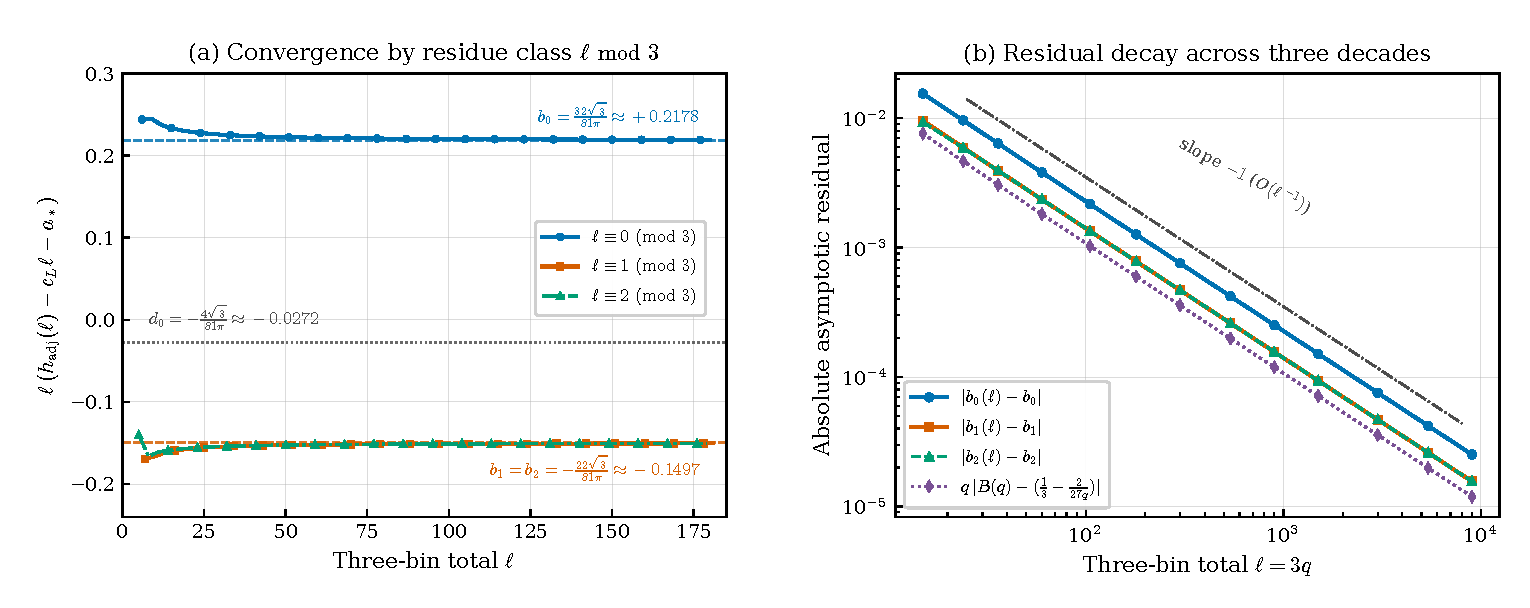
\includegraphics[width=\textwidth]{figures/fig1_residue_convergence.pdf}
  \caption{\textbf{Empirical verification of \cref{thm:main}.} (a) Exact sequence $\ell(\hadj(\ell)-c_L\ell-a_*)$ separated by residue class $\ell\bmod 3$, approaching the proved asymptotes $b_0=\frac{32\sqrt{3}}{81\pi}$ and $b_1=b_2=-\frac{22\sqrt{3}}{81\pi}$ around their mean $d_0=-\frac{4\sqrt{3}}{81\pi}$. (b) Log--log decay of $|b_r(\ell)-b_r|$ and the $1\mathrm{D}$ residual $q|B(q)-(\frac{1}{3}-\frac{2}{27q})|$ across three decades, confirming clean $O(\ell^{-1})$ convergence.}
  \label{fig:convergence}
\end{figure}

% =====================================================================
\section{Discussion, Practical Scope, and Methodology Note}
\label{sec:discussion}
% =====================================================================

\paragraph{Applied statistical scope.}
Discrete total variation goodness-of-fit testing (TVOR \cite{banic_elezovic_tvor} and the comb test \cite{banic_elezovic_ct}) targets ordered and circular histograms where alternating bin artifacts occur---including digital image forensics (quantization, contrast-stretching, and resampling comb patterns in $256$- to $65{,}536$-bin intensity histograms), analog-to-digital converter differential nonlinearity metrology, hardware random number generator verification, and periodic phase or circadian event histograms. In many such applications the bin-to-sample ratio $n/N$ is moderate rather than vanishingly small. Closing Conjecture~7.7 upgrades both the linear coefficient $\gamma(n)$ and the cyclic coefficient $\gamma_c(n)$ to unconditional closed-form theorems, enabling deterministic, simulation-free analytical moment calibration through $O(N^{-2})$ and supplying a rigorous quantitative diagnostic for when the fixed-$n$ expansion breaks down.

\paragraph{Methodological implications.}
From the viewpoint of asymptotic combinatorics and probability (cf.\ Diaconis and Zabell \cite{diaconis_zabell1991}, Bhattacharya and Rao \cite{bhattacharya_rao}), the principal lesson of the proof is that singular $\ell_1$ lattice functionals can sometimes be de-singularized \emph{before} taking asymptotics: by folding onto a Weyl chamber and telescoping exact factorial differences, a two-dimensional distributional problem at order $\ell^{-5/2}$ collapses into completely elementary one-dimensional Gaussian Euler--Maclaurin sums. Because the telescoping step \eqref{eq:inner-tel} relies only on linear weights and factorial absorption \eqref{eq:T-absorb}, analogous reductions are natural candidates for higher-order $1\mathrm{D}$ differences and non-uniform multinomial regimes in Parts~3--4 of \cite{banic_elezovic_p2}.

\paragraph{Limitations and verification boundary.}
We separate three epistemic layers explicitly. First, \cref{thm:main} (Conjecture~7.7: $b_0,b_1,b_2,d_0,\tri,\gamma_2$ and the cosine decomposition) is proved unconditionally from Mathlib primitives inside Lean~4 and re-checked across six independent proof kernels. Second, \cref{cor:unconditional}(i)--(iii) formalizes the exact algebraic simplifications of $\gamma(n)$, $\gamma_c(n)$, $\gamma(3;N)$, and $\gamma(4;N)$, while the upstream variance decompositions of \cite[Theorem~7.6, \S7.2, \S8]{banic_elezovic_p2} and \cite[Theorem~5.2]{banic_elezovic_p5} remain cited literature results outside our Lean kernel boundary, alongside the exact Python checks (\code{verify\_conjecture.py}). Third, this manuscript is an unreviewed independent preprint; although \code{Challenge.lean} ($143$ lines, Mathlib-only, Lean~4.35 \code{module} header) and \code{NonVacuity.lean} ($20$ witnesses) are designed for rapid third-party inspection alongside a live negative Lean kernel rejection check in CI, independent human line-by-line statement-fidelity sign-off remains open (tracked in \code{docs/statement-fidelity.md} and \code{formalization.yaml}).

\paragraph{Data, code availability, provenance, and export-control self-screen.}
All Lean~4 proofs, Python verification scripts, tests, figure generators, compiled PDFs, and byte-reproducible arXiv source bundles are publicly archived under dual open licenses (Apache-2.0 for code and Lean; CC-BY-4.0 for manuscript and documentation) at \href{https://github.com/0thernes/multinomial-tv-conjecture}{\nolinkurl{github.com/0thernes/multinomial-tv-conjecture}}; the interactive Lean~4 Blueprint is hosted at \href{https://0thernes.github.io/multinomial-tv-conjecture/blueprint/}{\nolinkurl{0thernes.github.io/multinomial-tv-conjecture/blueprint}}. Artifact integrity is anchored by \code{data/MANIFEST.sha256}, dual cryptographic timestamps (DigiCert RFC~3161 TSA \code{MANIFEST.sha256.tsr} and Bitcoin OpenTimestamps \code{MANIFEST.sha256.ots} under \code{data/}), and Sigstore SLSA build-provenance attestations emitted on public GitHub Actions CI. This work consists solely of published fundamental mathematical research in probability and statistics with zero cryptographic, military, or dual-use software (self-screened under EAR 15~CFR~734.8 and ITAR 22~CFR~120).

\paragraph{AI assistance, CRediT authorship, conflicts of interest, and errata policy.}
Alexander Stephen Donahue (Independent Researcher, Spokane, WA, USA; ORCID \code{0009-0006-8168-9648}) holds sole authorial responsibility (CRediT: Conceptualization, Methodology, Project Administration, Resources, Supervision, and Validation oversight). Interactive AI systems (Google Gemini / Antigravity) assisted with analytical exploration, Lean~4 formalization, Python test scaffolding, and manuscript preparation under human direction. Epistemic warrant rests solely on the reproducible six-kernel Lean~4 verification, independent exact/80-digit computation, and open-source artifacts. The author declares no competing financial or institutional interests and received no external funding. Version history, errata (including bibliographic fix \code{E-2026-001} restoring the five-digit suffix of \code{arXiv:2610.13366}), and our withdrawal commitment are recorded transparently in \code{CHANGELOG.md} and \code{ERRATA.md}.

\bibliographystyle{plainurl}
\bibliography{refs}

\end{document}
